\chapter{Related Works}
\label{relatedwork}

\section{Background Literature}
\label{relatedwork:background}

\subsection{Lucene Based Inverted Search Index}
An inverted index lists every unique word in any document and identifies all the documents each word occurs in. Since the late 1990s, search engines have been using an inverted index as the core structure to store and access information; Even Google, in its earlier stages, leveraged inverted indexes as means of accessing text documents for search\parencite{brin1998anatomy}. Sergey Brin and Larry Page partitioned web search engines to perform three critical tasks: Parsing, Indexing, and Ranking.

Opensource search engines such as the Apache Lucene\parencite{lucene2010apache} help provide hooks to index and rank documents for search. Lucene has become a popular search engine as many open-source search engines are built on top of Lucene to help simplify the access of the features of Lucene. Solr\footnote{https://solr.apache.org/}, Elasticsearch\footnote{https://www.elastic.co/elasticsearch/} as some opensource search engines built on top of Lucene. 

\subsubsection{Indexing With Lucene}
As Lucene leverages an inverted index to store information, it defines two fundamental units for indexing:
\begin{itemize}
    \item Document : A container for various Fields
    \item Field : Stores the terms that need to be indexed. It is key-value form of mapping. 
\end{itemize}
The Document allows for storing large hierarchical tree-like structures when indexing JSON objects. Every index consists of Documents. The index is similar to Database in the language of RDBMS. 

\subsection{Transformers and Machine Learning SOTA}
The Transformer model \parencite{vaswani2017attention} has recently proven to show SOTA performance on various domains ranging from natural language \parencite{brown2020language}, vision(\cite{radford2021learning}, \cite{dosovitskiy2020image}), music \parencite{huang2018music}, image-generation \parencite{ramesh2021zero} and even Web Table mining \parencite{deng2020turl}. These models can be trained with large amounts of data using self supervised training objectives \parencite{chen2020big}, \parencite{kolesnikov2019revisiting}, \parencite{goyal2019scaling}, \parencite{gidaris2018unsupervised}, \parencite{doersch2015unsupervised}. Once trained, these models can transfer their learning to different downstream tasks by making minor adjustments to their weights \parencite{howard2018universal} based on the task.  

\subsubsection{Transformer Architecture}
\begin{figure}[h]
    \centering
    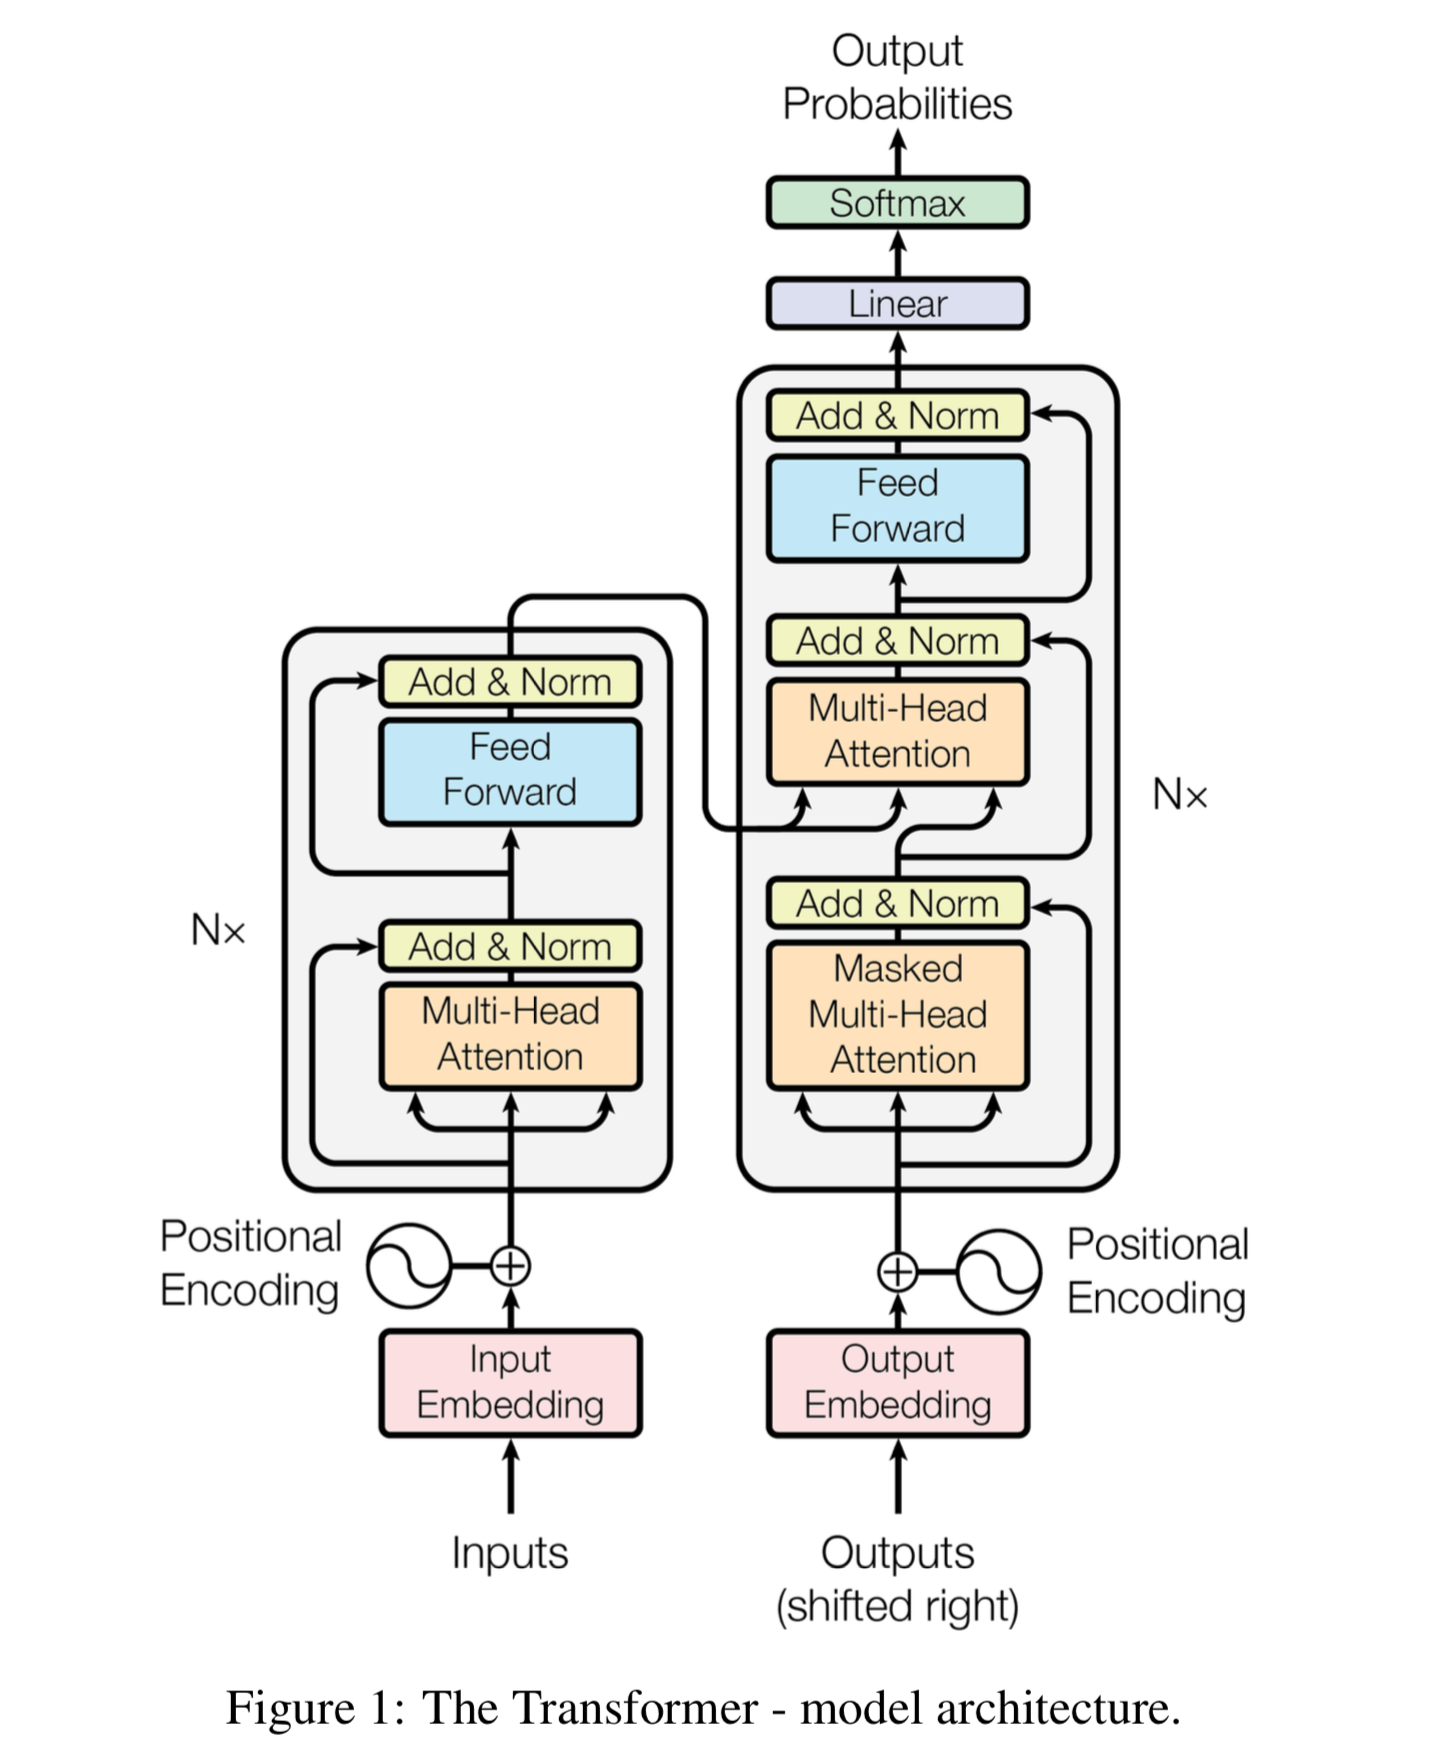
\includegraphics[width=0.7\maxwidth{\textwidth}]{src/images/transformer.png}
    \legend{\emph{Source}: From \cite{vaswani2017attention}}
    \caption{Transformer Architecture}
    \label{figure\arabic{figurecounter}}
\end{figure}
\refstepcounter{figurecounter}

The vanilla Transformer architecture \parencite{vaswani2017attention} was created for machine translation. The model consisted of an Encoder-Decoder Architecture using self-attention/cross-attention layers. The input to the transformer requires a sequence of symbols. The sequence of input and target symbols are created via a word piece tokenizer. The tokenized sequences are transformed into sequences of embeddings. Positional embeddings are added to the sequences, and then they are passed through either the encoder or decoder layer.

The self-attention/cross-attention layers consist of a multiheaded self-attention/cross-attention operation followed by pointwise feedforward layers with batch normalization \parencite{ioffe2015batch} and residual connections \parencite{he2016deep}. Multiple such layers are stacked together to create an encoder or decoder of the transformer. 

The encoder layer encodes a sequence into latent representations using the self-attention operation; the decoder layer decodes the latent representation from the encoder with the cross attention for language translation. Figure \ref{figure7} visualizes the operation of the encoder and decoder. 

Multiple variants of this architecture have been created such as the ones by \cite{radford2019language}, \cite{devlin2018bert}. The key insight behind the attention operation is provided in Section \ref{relatedwork:background:transformer:attention}, Section \ref{relatedwork:background:transformer:cross-attention}, 

\paragraph{Self-Attention}
\label{relatedwork:background:transformer:attention}
The self attention operation operates on a sequence $S \in \mathbb{R}^{s \times d}$ of $s$ length and $d$ dimensions. The self attention operation comprises three key components. A key matrix $K$, A query matrix $Q$, and value matrix $V$;each created from a linear transformation of $S$. 
$$A = softmax(\frac{QK^T}{\sqrt{d}})V$$

The $softmax(\frac{QK^T}{\sqrt{d}})$ operation creates a $s \times s$ dimensional matrix. Element ${i,j}$ in the matrix correspond to the weight of index $i$ in the sequence $S$ to index $j$ in sequence $S$. The operation is called self attention because the key matrix and the query matrix are derived from same sequence.

\paragraph{Cross Attention}
\label{relatedwork:background:transformer:cross-attention}
Self attention operation applies the attention opperation over the same sequence; Cross attention applies the attention operation over different sequences. The cross attention operates on a sequence $S_\alpha \in \mathbb{R}^{s \times d}$ and $S_\beta \in \mathbb{R}^{k \times d}$ where $S_\alpha$ is of $s$ length and $d$ dimensions and $S_\beta$ is of $k$ length and $d$ dimensions. The query matrix $Q_\alpha$ is created from a linear transformation of $S_\alpha$ and key matrix $K_\beta$, value matrix $V_\beta$ are created from a linear transformation of $S_\beta$. 

$$A_\alpha=softmax(\frac{Q_{\alpha}K_{\beta}^{T}}{\sqrt{d}})V_{\beta}$$

The $softmax(\frac{Q_{\alpha}K_{\beta}^{T}}{\sqrt{d}})$ operation creates a $s \times k$ dimensional matrix. Element ${i,j}$ in the matrix correspond to the weight of index $i$ in the sequence $S_\alpha$ to index $j$ in sequence $S_\beta$. This operation is useful in tasks such as language translation where the $S_\alpha$ can be a source language sentence and $S_\beta$ can be the target language sentence for translation.  

\subsubsection{Pretraining and Self Supervised Learning}
In NLP, Transformer models possess properties to scale and learn with massive amounts of data using generalized tasks such as language modeling or masked language modeling. The objective of language modeling is to predict the token $n+1$ given $n$ tokens in the sequence. The masked language modeling objective is to predict a masked out token in the sequence correctly given the other tokens. These training objectives allow the usage of large amounts of data from the web without going through the effort to clean the data. Recent State-of-the-art Language models such as GPT-3 \parencite{brown2020language} are trained using such self-supervised training objectives. 

\subsubsection{Advantages To Transfer Learning After Pretraining Models}
Recent studies such as the one by \cite{hernandez2021scaling}, showed that transformer models pretrained on large data with self-supervised learning objectives transfer learn better to downstream tasks with much less labeled data. The finetuning step\parencite{howard2018universal} of transfer learning involves adding a new linear layer and then training the model with small learning rates for the task-specific optimization. 


\subsubsection{Machine Learning For Tabular Data}
\cite{deng2020turl} recently applied structurally aware Transformers for self-supervised learning of web tables. The learned models possessed rich generalization capabilities for transfer into downstream tasks such as row filling based on headers, Entity Linking to the knowledge base, column type annotation etc. 

\section{Academic Research Search Engines}
\label{relatedwork:acad-search-engine}
\cite{gusenbauer2020academic} conducted an analysis of search engines based on criteria described in Table \ref{table1}.
The criteria described by \cite{gusenbauer2020academic} try to objectively evaluate the usefulness of a search engine to do systematic reviews.

\begin{table*}[h]
    \label{table\arabic{tablecounter}}
    \csvreader[%
     tabular={|p{7cm}|p{10cm}|},
            table head = \hline\textbf{Criteria} & \textbf{Meaning} \\\hline,
            late after line= \\\hline,
            late after last line=\\\hline %
            ]{searching-criteria-0.csv}{Criteria=\Criteria,Meaning=\Meaning}%
            {\Criteria & \Meaning}
            \centering
            \legend{\emph{Source}: From \cite{gusenbauer2020academic}}
            \caption{\label{tablecounter}Table explaining various criteria For Comparing Search Engines}
\end{table*}
\refstepcounter{tablecounter}

\begin{table*}[h]
    \label{table\arabic{tablecounter}}
    \csvreader[%
     tabular={|p{7cm}|p{10cm}|},
            table head = \hline\textbf{Criteria} & \textbf{Meaning} \\\hline,
            late after line= \\\hline,
            late after last line=\\\hline %
            ]{searching-criteria-1.csv}{Criteria=\Criteria,Meaning=\Meaning}%
            {\Criteria & \Meaning}
            \centering
            \legend{\emph{Source}: From \cite{gusenbauer2020academic}}
            \caption{\label{tablecounter}Table explaining various criteria for comparing search engines}
\end{table*}
\refstepcounter{tablecounter}

\begin{table*}[h]
    \label{table\arabic{tablecounter}}
    \csvreader[%
     tabular={|p{7cm}|p{10cm}|},
            table head = \hline\textbf{Criteria} & \textbf{Meaning} \\\hline,
            late after line= \\\hline,
            late after last line=\\\hline %
            ]{searching-criteria-2.csv}{Criteria=\Criteria,Meaning=\Meaning}%
            {\Criteria & \Meaning}
            \centering
            \legend{\emph{Source}: From \cite{gusenbauer2020academic}}
            \caption{\label{tablecounter}Table explaining various criteria for comparing search engines}
\end{table*}
\refstepcounter{tablecounter}

% Recent studies have tried to compare various search engines, finding causes for search failures and 
% recommend feature to improve search precision. 


\cite{li2017investigating} performed a detailed analysis on the patterns and failures in search for academic search. 
Their analysis concluded that search queries in academic search had substantially more entity-based queries than web search and 
null queries attributed to a significant fraction of failures, i.e., search engine found no search results. 
This analysis is quite helpful in correlating the need for a "Controlled Vocabulary"(Table \ref{table1}) in search to improve precision. 

\cite{kacem2018analysis} analyzed the improvement of search precision based on the usage of \textit{search stratagems}.
Search stratagems are additional filters along with the search terms. They provide further context around filtering a search query. 
Some examples of such filters can Authors of a paper, Forward Citation Search, Footnote Chasing, etc.
The study by \cite{kacem2018analysis} concluded that search stratagems could improve search precision for the search queries.

\cite{rovira2019ranking} conducted a study to analyze the impact of citation count on ASEO(Academic Search Engine Optimization). 
Their study concluded that Microsoft Academic and Google Scholar seem to leverage received citations as a part of the relevance 
ranking algorithm. This study also noted many unknown attributes in the relevance ranking algorithms for Google Scholar and Microsoft Academic.


\section{Academic Research Literature Mining}
\label{relatedwork:acad-lit-mining}
Academic Literature mining has many applications such as document structure analysis, citation analysis, document summarization, table extraction, and more. Deep learning-based methods dominate many of the recent SOTA academic literature mining methods. 

\cite{beltagy2019scibert} created Sci-Bert by training a BERT model \parencite{devlin2018bert} using a large corpus of research data. Sci-Bert can be finetuned for downstream tasks such as citation intent detection, relation extraction, and even named entity detection. 
 
\cite{safder2020deep} leveraged deep learning techniques extract metadata from research documents. \cite{zha2019mining} proposed methods to track the evolution of algorithms and techniques to make research more understandable. 

Table extraction and parsing have also seen a lot of recent advancements. Methods either work on PDF-based documents or LaTeX based documents.  Some such advances can include \cite{milosevic2019framework}'s framework for extracting tables from biomedical literature articles or \cite{kardas2020axcell}'s methods for extracting tables describing SOTA comparisons from machine learning papers. 

All of these advances are because of curation and opensource availability to many datasets some of such being Arxiv Tables\footnote{http://boston.lti.cs.cmu.edu/eager/table-arxiv/} or Semantic Scholar Open Research Corpus\parencite{ammar-etal-2018-construction} or the Sci-Cite dataset \parencite{cohan2019structural} or the PaperWithCode datasets\footnote{https://paperswithcode.com/}.


\section{Types Of Tables in Scientific Research}
\label{relatedwork:table-type}
Earlier work done by \cite{kim2012scientific} defined the types of tables based on their content and purpose. \cite{kim2012scientific} sampled 25 papers from the domains of CS, Biomedical, Life Science, Chemistry, Material Science, Electrical Engineering and Medicine chose to define the following types of tables for scientific documents:
\begin{itemize}
    \item \textbf{Definition Table} : \textit{These tables describe equation definitions or symbol definitions}
    \item \textbf{Statistics Table} : \textit{These tables describe some statistical distribution which is not related to experiment results}
    \item \textbf{Survey Table } : \textit{These tables describe questionaire surveys and results }
    \item \textbf{Example Table } : \textit{These tables provide emphasis of something that needs to be clearly explained }
    \item \textbf{Procedure Table} : \textit{These tables describe a flow or a process}
    \item \textbf{Experiments Setting Table } : \textit{These tables describe some experiment parameters}
    \item \textbf{Experiments Results Table } : \textit{These tables describe the results of some experiments discussed in the paper.}
\end{itemize}

\cite{kim2012scientific} also found that most of the tables in scientific documents describe results from experiments based on the samples they annotated. 



